\documentclass{beamer}
\usepackage{siunitx,booktabs,xcolor,xspace,multirow,graphicx,lipsum}
\usepackage[spanish,mexico,es-noindentfirst]{babel}
\usepackage[utf8]{inputenc}
\usepackage{tikz}
\usepackage{tikzsymbols}
\usepackage{subcaption}
\usepackage{charter}
\usetheme{Madrid}
\usepackage{tcolorbox}
\usepackage{hyperref}
\usepackage{animate}
\usepackage{transparent}

\usepackage[T1]{fontenc}
\usepackage[export]{adjustbox}
\usetikzlibrary{positioning}
\usefonttheme{serif}
\DeclareUnicodeCharacter{2212}{\textendash}

\setbeamertemplate{frametitle}{
	\begin{beamercolorbox}[wd=\paperwidth, ht=0.85cm, sep=0.25cm]{frametitle}
		\begin{tikzpicture}[remember picture,overlay]
			\node[anchor=north east] at (current page.north east) {\includegraphics[height=0.65cm]{fig/aries.png}};
		\end{tikzpicture}
		\usebeamerfont{frametitle}\bfseries\insertframetitle
	\end{beamercolorbox}
}
\definecolor{lightshadygreen}{RGB}{204, 230, 255}
\setbeamercovered{transparent}
\setbeamertemplate{caption}[numbered]
\setbeamercolor{frametitle}{bg=lightshadygreen,fg=black}
\setbeamercolor{author in head/foot}{bg=lightshadygreen,fg=blue}
\setbeamercolor{title in head/foot}{bg=lightshadygreen,fg=blue}
\setbeamercolor{date in head/foot}{bg=lightshadygreen,fg=blue}
\setbeamercolor{titlelike}{parent=structure,bg=lightshadygreen,fg=black}
\setbeamertemplate{section in toc}[sections numbered]
\setbeamertemplate{subsection in toc}[subsections numbered]
\setbeamerfont{section in toc}{series=\bfseries}
\setbeamercolor{section in toc}{fg=black}
\setbeamercolor{caption name}{fg=black}
\setbeamerfont{caption name}{series=\bfseries}
\setbeamerfont{caption}{size=\small}
\setbeamercolor{bibliography entry author}{fg=black}
\setbeamercolor{bibliography entry title}{fg=black} 
\setbeamertemplate{section in toc}{\inserttocsectionnumber.~\inserttocsection\par}
\setbeamertemplate{subsection in toc}{\hspace{1.5em}\inserttocsectionnumber.\inserttocsubsectionnumber~\inserttocsubsection\par}

% Apply the custom color to the frametitle
\setbeamercolor{frametitle}{bg=lightshadygreen, fg=black}

\title[\textbf{Talk at Research Campus Waischenfeld}]{\textbf{When SPH meets SII \\ \small{Numerical Hydrodynamics for Close Binary Star Systems}}}
\author[\textbf{Km Nitu Rai}]{Prasenjit Saha, Subrata Sarangi and Km Nitu Rai \vspace{0.01cm} \\ 
	{\scriptsize \underline{\textcolor{blue}{niturai201296@gmail.com}}} \\
	{\scriptsize \underline{\textbf{\tiny Presenting at}}} \\	
	{\scriptsize \underline{\textcolor{blue}{Stellar Intensity Interferometry Workshop 2026}}}\\
	{\scriptsize \underline{\textcolor{blue}{5-9 Oct 2026, Research Campus Waischenfeld (Germany) of the Fraunhofer Society}}}
}

\date{\vspace{-5cm}\textbf{6th October 2026}}

\renewcommand{\maketitle}{
	\begin{figure}[!htb]
		\centering
		\includegraphics[height=1cm]{fig/UZH.png}\hfill
		\includegraphics[height=1cm]{fig/CUTM.png}\hfill
		\includegraphics[height=1cm]{fig/aries.png}
	\end{figure}
	\vspace{-1cm}
	\titlepage
}



\newcommand{\rotx}{\mathop{\mathsf{X}}\nolimits}
\newcommand{\roty}{\mathop{\mathsf{Y}}\nolimits}
\newcommand{\rotz}{\mathop{\mathsf{Z}}\nolimits}
\renewcommand{\pmatrix}[1]{\left[\begin{matrix}#1\end{matrix}\right]}


\definecolor{beamer_color}{RGB}{176,196,222} 
\begin{document}
	\maketitle
	\begin{frame}
		\centering
		\vfill
		
		{\Large\bfseries\textcolor{red}{Beyond the Point-Source Approximation}}\\[0.7cm]
		
		{\Large
			\textcolor{blue}{\textit{No more privileges.}}\\[0.25cm]
			\textcolor{blue}{\textit{No more idealized uniform stellar disk.}}
		}\\[0.8cm]
		
		\rule{0.55\textwidth}{1pt}\\[0.5cm]
		
		{\Large\bfseries
			\textcolor{red}{Time to deal with real sources.}
		}
		
		\vfill
		\begin{tikzpicture}[remember picture,overlay]
			\node[anchor=south east, xshift=-0.2cm, yshift=0.8cm] 
			at (current page.south east) 
			{\tiny \textbf{\textcolor{blue}{Philip Mocz, 2011, MNRAS, 10(1), 1-9}}};
		\end{tikzpicture}
	\end{frame}

    \begin{frame}{From Point to Extended Source}
    	\begin{columns}[c]
    		\column{0.65\textwidth}
    		\begin{itemize}
    			\item A star is a collection of particles - \textbf{FLUID}.    			
    			\item Particle's mass in a volume - \textbf{DENSITY}    			
    			\item Density determines the \textbf{pressure} through
    			the polytropic equation of state
    			\[
    			P = K\rho^\gamma.
    			\]    			
    			\item It forms a \textbf{finite, spatially extended source}
    			rather than a point source.
    		\end{itemize}    		
    		\column{0.35\textwidth}
    		\begin{figure}
    			\centering
    			\animategraphics[autoplay, loop, width=\linewidth]{5}{fig/frames_single/single_star}{1}{31}
    			\caption*{\small Extended stellar surface}
    		\end{figure}
    	\end{columns}
    \end{frame}


    \begin{frame}
     	\centering
	    \vfill	
	    {\Large\textbf{How Do We Study an Extended Source and Signal?}}	
	    \textbf{\textcolor{blue}{THE PARTICLES}}	
	    
	    \vspace{0.5cm}	
	    {\color{blue}\rule{0.25\textwidth}{1.5pt}}    
	    \hspace{0.15cm}
	    {\color{red}\textbf{\Large Smoothed Particle Hydrodynamics}}
	    
	    \hspace{0.15cm}
	    {\color{blue}\rule{0.25\textwidth}{1.5pt}}	
    	\vfill
    \end{frame}

    \begin{frame}{Equilibrium: The Balancing Force}   	
    	\begin{columns}[c]    		
    		\column{0.65\textwidth}    		
    		\begin{itemize}
    			\item Equilibrium - \textbf{pressure balances gravity}.    			
    			\item The pressure gradient provides an outward force:
    			\[
    			\mathbf{a}_{P}
    			=-\frac{1}{\rho}\nabla P
    			\]    			
    			\item Gravity provides an inward acceleration:
    			\[
    			\mathbf{a}_{G}=-\nabla\Phi
    			\]   			
    			\item At equilibrium:
    			\[
    			\boxed{\mathbf{a}_{P}+\mathbf{a}_{G}=0}
    			\]
    		\end{itemize}    		
    		\column{0.35\textwidth}    		
    		\centering
    		\begin{tikzpicture}[>=stealth, scale=0.85]    			
    			\shade[ball color=orange!60] (0,0) circle (1.5);
    			
    			\draw[->, thick, blue] (0,1.5) -- (0,0.65);
    			\draw[->, thick, blue] (0,-1.5) -- (0,-0.65);
    			\draw[->, thick, blue] (1.5,0) -- (0.65,0);
    			\draw[->, thick, blue] (-1.5,0) -- (-0.65,0);
    			
    			\draw[->, thick, red] (0.65,0.2) -- (1.8,0.2);
    			\draw[->, thick, red] (-0.65,0.2) -- (-1.8,0.2);
    			\draw[->, thick, red] (0.2,0.65) -- (0.2,1.8);
    			\draw[->, thick, red] (0.2,-0.65) -- (0.2,-1.8);
    			
    			\node[blue] at (0,-2.0) {\scriptsize Gravity};
    			\node[red] at (2.0,0.45) {\scriptsize Pressure};
    			
    			\node at (0,0) {\textbf{Star}};    			
    		\end{tikzpicture}    		
    	\end{columns}    	
    \end{frame}

    \begin{frame}{Local Neighbourhood}
    	\begin{columns}[c]
    		\column{0.65\textwidth}    		
    		\begin{itemize}
    			\item Estimate the properties using	\textbf{Local Neighbourhood} of particles.    			
    			\item \textbf{Smoothing Length} $h$ sets the size of it.   			
    			\item A kernel distributes the contribution of \textbf{each particle smoothly}:
    			\begin{equation*}
    				W(r,h)
    				=
    				\frac{1}{\pi^{3/2}h^3}
    				\exp\left(-\frac{r^2}{h^2}\right).
    			\end{equation*}
    			\begin{equation*}
    				\int W(r,h)\,d^3r = 1.
    			\end{equation*}
      		    \item Particles closer to the point of interest contribute
    		    \textbf{more strongly}.
    		\end{itemize}   		
    		\column{0.35\textwidth}
    		\begin{figure}
    			\centering
    			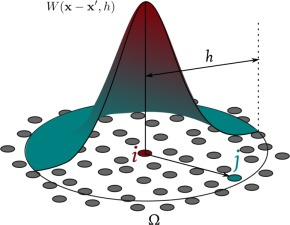
\includegraphics[width=\textwidth]{fig/Gauss_Kernal.jpg}
    			\caption*{\tiny \textbf{Gaussian smoothing kernel}}
    		\end{figure}
    	\end{columns}
    \end{frame}

    \begin{frame}{Evolution of Particle}	
    	\begin{columns}[c]		
		    \column{0.6\textwidth}		
		    \begin{itemize}
			    \item Particles are evolved using the \textbf{leap-frog method}.			
		       	\item Velocity is updated by a half-step:
			    \begin{equation*}
			    	\mathbf{v}_i^{n+1/2} = 	\mathbf{v}_i^n + \frac{\Delta t}{2}\mathbf{a}_i^n
			    \end{equation*}			
		    	\item Position is updated by a full step:
			    \begin{equation*}
			    	\mathbf{r}_i^{n+1} = \mathbf{r}_i^n	+ \Delta t\,\mathbf{v}_i^{n+1/2}
			    \end{equation*}			
			    \item Acceleration is then recomputed for the next step.
	    	\end{itemize}		
		    \column{0.4\textwidth}		
		    \centering
		    {\color{blue}\Large\textbf{Leap-Frog}}		
		    \vspace{0.3cm}		
		    \begin{tikzpicture}[>=stealth, scale=0.8, every node/.style={font=\small}]			
		    	\draw[->, thick] (0,0) -- (5,0) node[right] {$t$};			
			    \fill[red] (0.8,0) circle (3pt);
	    		\fill[red] (4.2,0) circle (3pt);			
	    		\node[red, above] at (0.8,0) {$\mathbf r_i^n$};
    			\node[red, above] at (4.2,0) {$\mathbf r_i^{n+1}$};			
    			\draw[blue, thick, ->] (2.5,0.2) -- (2.5,1.1);			
	    		\node[blue, above] at (2.5,1.1)
	    		{$\mathbf v_i^{n+1/2}$};			
	    		\draw[red, thick, ->] (1,-0.35) -- (4,-0.35);			
	    		\node[red, below] at (2.5,-0.35)
	    		{\scriptsize $\Delta t$};			
	    	\end{tikzpicture}		
		    \vspace{0.3cm}
		
		    \begin{block}{Key idea}
		    	\centering
		    	{\color{red}$\mathbf r$: full steps}
	    		\qquad
	    		{\color{blue}$\mathbf v$: half steps}
	    	\end{block}		
    	\end{columns}	
    \end{frame}

    \begin{frame}
    	\centering
    	\vfill	
    	{\Large\textbf{Extend the Idea to the Close Binary Star System}}
    		
    	\textbf{\textcolor{blue}{THE MODELING PROBLEM OF COMPLEX SYSTEM}}	
    	
    	\vspace{0.5cm}	
    	{\color{blue}\rule{0.25\textwidth}{1.5pt}}    
    	\hspace{0.15cm}
    	{\color{red}\textbf{\Large In Absence of Analytical Equations}}
    	
    	\hspace{0.15cm}
    	{\color{blue}\rule{0.25\textwidth}{1.5pt}}	
    	\vfill
    \end{frame}

    \begin{frame}{Why a Close Binary Star System?}
    	
    	\begin{itemize}
    		\item The gravitational field is no longer spherically symmetric.
    		
    		\item The stars can undergo strong tidal interaction.
    		
    		\item Their surfaces can become distorted from spherical symmetry.
    		
    		\item The observed brightness distribution changes with orbital phase.
    	\end{itemize}
    	
    	\begin{block}{Key Idea}
    		\centering
    		A binary system requires the \textbf{dynamics and surface structure}
    		to be evolved together.
    	\end{block}
    	
    \end{frame}

    \begin{frame}{Representing the Binary with SPH Particles}   	
    	\begin{itemize}
    		\item Each star is represented by a collection of SPH particles, which carries:
    		\[
    		m_i,\quad \mathbf r_i,\quad \mathbf v_i,\quad
    		\rho_i,\quad u_i,\quad h_i
    		\]
    		
    		\item The particles interact through:
    		\begin{itemize}
    			\item gravitational force,
    			\item pressure force,
    			\item hydrodynamic interactions.
    		\end{itemize}
    	\end{itemize}
    	
    	\begin{block}{Advantage}
    		\centering
    		The stellar surface does not need to be prescribed analytically.
    	\end{block}    	
    \end{frame}

    \begin{frame}{Initial Binary Configuration}
    	\begin{columns}[c]
    		\column{0.6\textwidth}
    		\begin{itemize}
    			\item Two relaxed polytropic stars in a orbit.
    			\item Orbital separation is set by the chosen binary parameters.
    			\item Initial velocities provide the orbital motion.
    			\item At each time step:
    			\begin{enumerate}
    				\item Particle positions are updated.
    				\item Velocities are updated.
    				\item Density and pressure are recalculated.
    				\item Gravitational and hydrodynamic forces are evaluated.
    			\end{enumerate}
    		\end{itemize}
    		
    		\begin{equation*}
    			\mathbf a_i =
    			\mathbf a_{i,\mathrm{grav}}
    			+
    			\mathbf a_{i,\mathrm{pressure}}
    		\end{equation*}
    		
    		\column{0.4\textwidth}
    		\begin{figure}
    			\animategraphics[autoplay, loop, width=\linewidth]{5}{fig/frames_binary/binary_star}{1}{71}
    		\end{figure}
    	\end{columns}    	
    \end{frame}

    \begin{frame}{The Projected Surface and Signal}
    	\centering
    	\begin{figure}
    		\animategraphics[autoplay, loop, width=\linewidth]{5}{fig/frames_signal_binary/binary_signal}{1}{71}
    		\caption*{The binary star, its projected surface and signal on earth.}
    	\end{figure}
    \end{frame}

	\begin{frame}{}
		\begin{center}
			{\fontsize{40}{50}\selectfont \underline{Thank You!!}}
		\end{center}
	\end{frame}

\end{document}